% ==============================================================================
% CHƯƠNG 2 - PHẦN B: TÍCH HỢP, KHỬ TRÙNG LẶP VÀ ĐIỀU PHỐI (INTEGRATE)
% ==============================================================================

\section{Hợp Nhất Lược Đồ Đa Nguồn và Kho Lưu Trữ Bất Biến Bronze}
\label{sec:ch2_integrate}

\subsection{Lưu Trữ Bất Biến Tầng Bronze và Bản Ghi Minh Họa}
\label{sec:ch2_bronze}

Trước khi bất kỳ phép biến đổi cấu trúc nào diễn ra, hàm \path{QueueConsumer._bronze()} (\path{src/ingestion/queue_consumer.py}) lưu nguyên bản payload JSON nhận từ hàng đợi vào đường dẫn \path{bronze/papers/{year}/{paper_id}.json} (cùng bản HTML gốc nếu có sẵn trong thông điệp) trên MinIO S3. Thất bại ở bước ghi Bronze sẽ lập tức hủy xử lý bài báo trong lô hiện tại, bảo đảm \textbf{Bất biến Nguồn gốc Thô (\textit{Immutable Raw Invariant})} phục vụ kiểm tra chéo và tái xử lý.

Trong kho Bronze, siêu dữ liệu thô phản ánh đặc thù từng nguồn. Hình~\ref{fig:bronze_raw_capture} minh họa một bản ghi OpenAlex được mở trực tiếp từ kho qua Explorer (\path{bronze/tier1/openalex_W2001598892.json}), cho thấy một số trường có thể khuyết như \texttt{abstract}, \texttt{authors}, hoặc \texttt{arxiv\_id}; đây là ví dụ minh họa cấu trúc thô, không dùng để suy diễn tỷ lệ thiếu dữ liệu của toàn bộ kho Bronze. Do tính dị thể này, tầng tích hợp không giả định mọi nguồn đều đầy đủ các trường mà thực hiện ánh xạ phòng thủ tại \texttt{SilverLakehouseWriter.prepare\_record()} và \texttt{\_normalize\_frame()} (\path{src/transformation/silver_writer.py}).

\begin{figure}[!htbp]
  \centering
  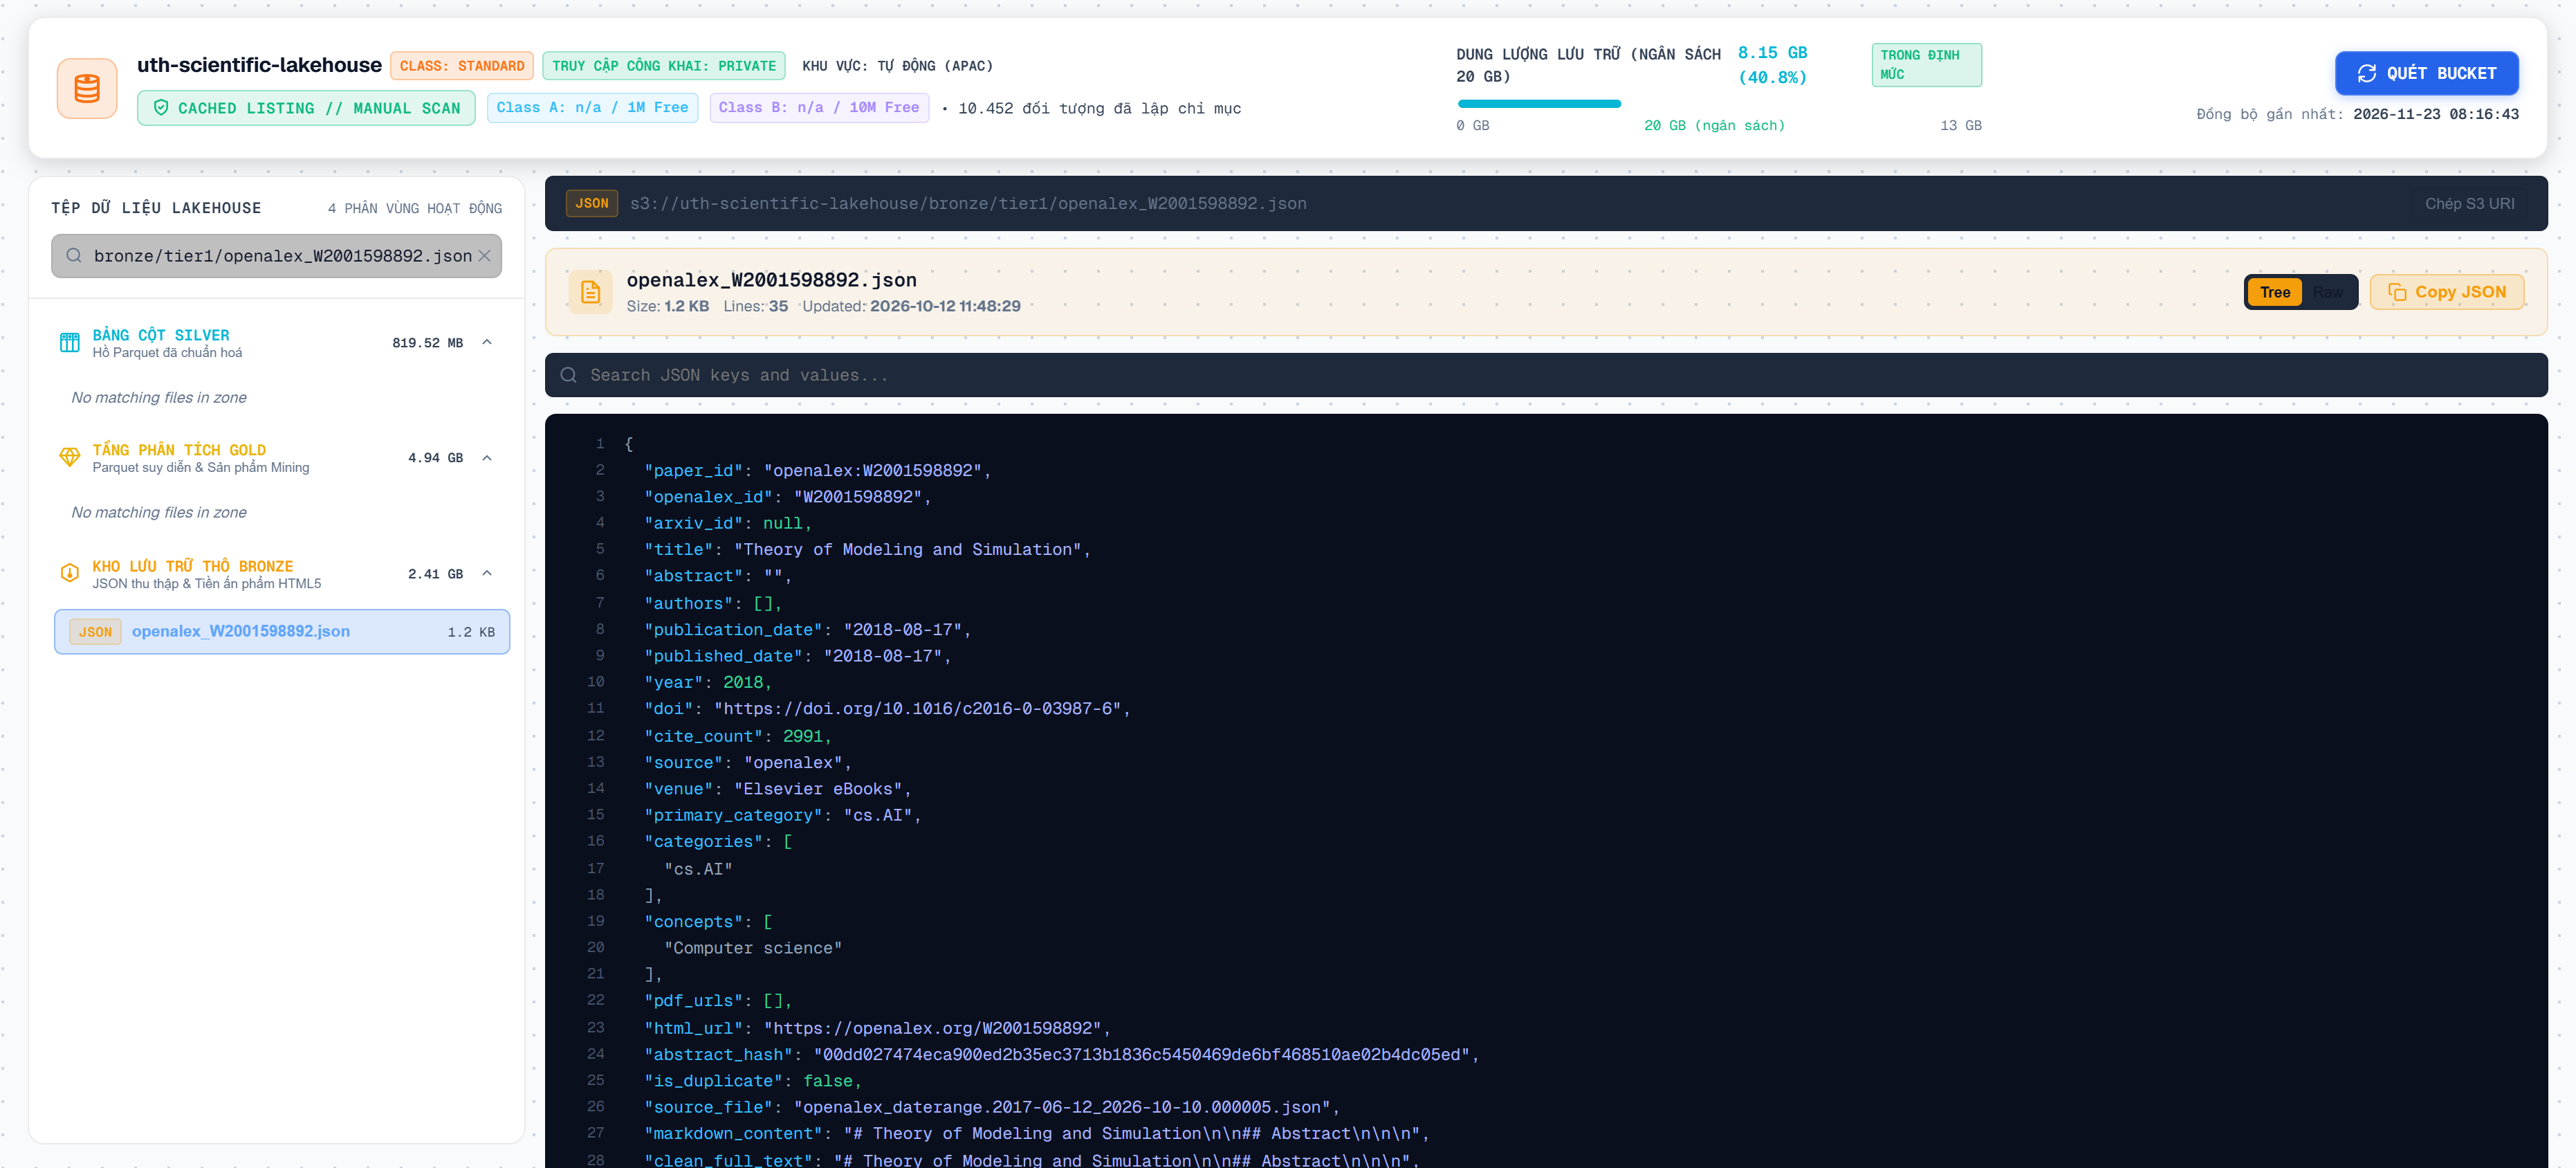
\includegraphics[width=\linewidth,height=0.62\textheight,keepaspectratio]{figures/captured_20261123_082337/02_bronze_raw_metadata.png}
  \caption[Ví dụ bản ghi metadata thô Bronze trên Explorer]{Ví dụ bản ghi metadata thô Bronze trên Explorer}
  \ReportNote{Nguồn: Cấu trúc bản ghi siêu dữ liệu thô lưu trữ dưới định dạng JSON trên kho MinIO Object Storage (\path{bronze/tier1/openalex_W2001598892.json}), chụp ngày 23/11/2026.}
  \label{fig:bronze_raw_capture}
\end{figure}

\subsection{Lược Đồ Chuẩn Hóa 23 Cột Tầng Silver Papers}
\label{sec:ch2_silver_schema}

Mọi bản ghi đến từ arXiv RSS/OAI-PMH, CVF HTML, Semantic Scholar JSON hay dữ liệu kế thừa (OpenReview, OpenAlex, Zenodo) đều được ép kiểu chặt chẽ về lược đồ chuẩn gồm \textbf{23 trường cột} trong \texttt{SilverLakehouseWriter.SCHEMA}. Bảng~\ref{tab:silver_schema} trình bày đầy đủ tên cột, kiểu Apache Arrow, quy tắc điền khuyết/chuẩn hóa và vai trò hạ nguồn của bảng \path{silver/papers/year=YYYY/}.

\begingroup
\small
\setlength{\tabcolsep}{3.5pt}
\setlength{\LTpre}{0pt}
\setlength{\LTpost}{4pt}
\begin{longtable}{|>{\centering\arraybackslash}p{8mm}|>{\raggedright\arraybackslash}p{28mm}|>{\raggedright\arraybackslash}p{22mm}|>{\raggedright\arraybackslash}p{44mm}|>{\raggedright\arraybackslash}p{38mm}|}
\caption[Lược đồ chuẩn hóa 23 cột của bảng Silver Papers]{Lược đồ chuẩn hóa 23 cột của bảng \texttt{silver/papers/} (\texttt{SilverLakehouseWriter.SCHEMA})}
\label{tab:silver_schema}\\
\hline
\textbf{STT} & \textbf{Tên cột} & \textbf{Kiểu Arrow} & \textbf{Quy tắc chuẩn hóa / Giá trị mặc định} & \textbf{Nguồn gốc \& Vai trò hệ thống} \\
\hline
\endfirsthead
\multicolumn{5}{l}{\small Bảng \thetable{} (tiếp theo)}\\
\hline
\textbf{STT} & \textbf{Tên cột} & \textbf{Kiểu Arrow} & \textbf{Quy tắc chuẩn hóa / Giá trị mặc định} & \textbf{Nguồn gốc \& Vai trò hệ thống} \\
\hline
\endhead
\hline
\multicolumn{5}{r}{\small (Còn tiếp ở trang sau)}\\
\endfoot
\hline
\endlastfoot
1 & \path{paper_id} & \path{pa.string()} & Ép chuỗi chuẩn hóa (vd. \texttt{2401.01234}, \path{cvf_*}, \path{s2_*}) & Khóa định danh chính dùng khử trùng \& phân mảnh \\
\hline
2 & \path{abstract_hash} & \path{pa.string()} & SHA-256 (64 hex) của \path{abstract}; nếu rỗng dùng \path{title} & Khóa khử trùng nội dung liên nguồn \\
\hline
3 & \path{doi} & \path{pa.string()} & Có thể \texttt{None} nếu nguồn không cung cấp & Liên kết chuẩn trích dẫn học thuật \\
\hline
4 & \path{journal_ref} & \path{pa.string()} & Tên hội nghị/tạp chí (vd. \texttt{CVPR2024}, \path{venue} S2); có thể \texttt{None} & Ngữ cảnh xuất bản \\
\hline
5 & \path{title} & \path{pa.string()} & Ưu tiên \path{parsed_title} từ HTML, fallback \path{raw_meta["title"]} & Tiêu đề bài báo làm sạch \\
\hline
6 & \path{abstract} & \path{pa.string()} & Ưu tiên \path{parsed_abstract}, fallback \path{raw_meta["abstract"]} & Nội dung tóm tắt chuẩn \\
\hline
7 & \path{authors} & \path{pa.list_(pa.string())} & Chuẩn hóa iterable thành danh sách chuỗi tên tác giả & Đầu vào mạng đồng tác giả PageRank / Louvain \\
\hline
8 & \path{categories} & \path{pa.list_(pa.string())} & Danh sách đầy đủ các nhãn ngành; chuyển scalar thành \texttt{[str]} & Đầu vào giao dịch FP-Growth \& \path{category_count} \\
\hline
9 & \path{primary_category} & \path{pa.string()} & Lấy \path{raw_meta["primary_category"]}, fallback \path{categories[0]} hoặc \texttt{"unknown"} & Phân tầng EDA, Trend Velocity \& lọc Qdrant \\
\hline
10 & \path{published_date} & \path{pa.string()} & Chuỗi ISO 8601 hoặc \texttt{YYYY-MM} / \texttt{YYYY} theo quy tắc OAI/CVF/S2 & Phân vùng theo năm (\path{year=YYYY}) \& thị phần theo tháng \\
\hline
11 & \path{crawled_at} & \path{pa.string()} & Thời điểm thu thập UTC ISO 8601 từ DAG/Harvester & Truy vết độ trễ thu thập \\
\hline
12 & \path{pdf_url} & \path{pa.string()} & URL tệp PDF gốc (arXiv, CVF, hoặc \path{openAccessPdf} của S2) & Nguồn dự phòng cho Tier 3 ngoài arXiv \\
\hline
13 & \path{html_url} & \path{pa.string()} & URL bản HTML5 / landing page (rỗng nếu không có) & Nguồn chính cho bóc tách LaTeXML \\
\hline
14 & \path{total_sections} & \path{pa.int64()} & Tổng số mục cấu trúc bóc tách được (\path{len(sections)}) & Quality Gate ($\ge 2$) \& Chỉ dấu làm giàu \\
\hline
15 & \path{total_math_count} & \path{pa.int64()} & Số phần tử toán \texttt{<math>} / \path{ltx_Math} parser đếm được & EDA \& Đặc trưng Isolation Forest \\
\hline
16 & \path{total_words} & \path{pa.int64()} & Tổng số từ toàn văn (hoặc fallback đếm từ \path{clean_full_text}) & Quality Gate ($\ge 300$) \& Đặc trưng Isolation Forest \\
\hline
17 & \path{sections_json} & \path{pa.string()} & Chuỗi JSON UTF-8 (\path{ensure_ascii=False}) lưu mảng đối tượng section & Đầu vào cho \texttt{AcademicChunker} tầng 2 \\
\hline
18 & \path{clean_full_text} & \path{pa.string()} & Văn bản liên tục ghép Title, Abstract và các mục \texttt{\#\# \{title\}} & Văn bản chuẩn cho phân đoạn tầng 3 \& kiểm tra \\
\hline
19 & \path{transformed_at} & \path{pa.string()} & Thời điểm UTC ISO 8601 khi tạo bản ghi Silver & Nhật ký chuyển đổi \\
\hline
20 & \path{cite_count} & \path{pa.int64()} & Lấy \path{cite_count} hoặc \path{citation_count}, điền khuyết \texttt{0} & Xếp hạng Semantic Scholar \& EDA tương quan \\
\hline
21 & \path{source} & \path{pa.string()} & Mặc định \texttt{"arxiv"} (\path{arxiv_rss_realtime}, \path{cvf}, \path{semantic_scholar}, \ldots) & Truy vết nhà cung cấp \\
\hline
22 & \path{tier} & \path{pa.string()} & Mặc định \texttt{"tier1"} (\texttt{tier1}, \texttt{tier2}, \texttt{tier3}) & Phân tách tầng thu thập trong cùng bảng Silver \\
\hline
23 & \path{content_origin} & \path{pa.string()} & \path{arxiv_html5}, \path{ar5iv_html5}, \path{cached_html}, \path{open_access_pdf}, \path{abstract_fallback}, \path{abstract_only} & Kiểm toán nguồn gốc bóc tách nội dung \\
\hline
\end{longtable}
\ReportNote{Nguồn: Đặc tả 23 trường Apache Arrow tại \path{src/transformation/silver_writer.py} (\texttt{SilverLakehouseWriter.SCHEMA}, \texttt{prepare\_record()}, \texttt{\_normalize\_frame()}) và \path{unified_content_resolver.py} (kiểm chứng trên commit \texttt{f421707}/\texttt{aae74de} ngày 25/11/2026); giúp DuckDB S3 và \texttt{AcademicChunker} đọc thống nhất mọi nguồn dị thể.}
\endgroup


\section{Lá Chắn Khử Trùng Lặp Hai Tầng (Deduplication Shield)}
\label{sec:ch2_dedup}

Một bài báo khoa học thường xuất hiện nhiều lần dưới các định danh khác nhau (ví dụ \texttt{2401.01234v1} so với \texttt{2401.01234v2}, hoặc một công trình xuất hiện đồng thời trên CVF, arXiv và Semantic Scholar). Lá chắn khử trùng lặp được cài đặt đồng bộ tại cả phía Producer (\path{dags/_common.py}) và phía Consumer (\path{src/storage/known_papers.py} kết hợp \path{src/utils/hasher.py}) theo quy trình hai tầng độc lập:
\begin{enumerate}[label=\textbf{\arabic*.}]
  \item \textbf{Nhánh vượt chốt (\texttt{refresh == True})}: Nếu thông điệp mang cờ làm mới (như từ \texttt{dag\_tier3\_pdf\_backfill}), hệ thống bỏ qua bước chặn trùng ở Silver để cho phép bóc tách lại toàn văn giàu hơn và cập nhật đè vector trên Qdrant.
  \item \textbf{Tầng A --- Chuẩn hóa Định danh}: Rút gọn mã phiên bản qua \path{normalize_id(paper_id)} và kiểm tra trong tập \texttt{known} lẫn tập \texttt{in\_batch} hiện hành; nếu trùng, loại bỏ ngay.
  \item \textbf{Tầng B --- Dấu vân tay Nội dung SHA-256}: Nếu chưa trùng ID, tính \texttt{abstract\_hash} sau khi chuẩn hóa văn bản 5 bước; nếu khác rỗng và xuất hiện trong \texttt{known} hoặc \texttt{in\_batch}, loại bỏ do trùng nội dung liên nguồn; ngược lại ghi nhớ qua \texttt{remember()} và cho phép xử lý Bronze/Silver.
\end{enumerate}

\subsection{Tầng A: Chuẩn Hóa Định Danh (\texttt{normalize\_id})}
\label{sec:ch2_dedup_id}

Hàm \texttt{normalize\_id} (\path{src/storage/known_papers.py}) loại bỏ hậu tố phiên bản ở cuối chuỗi định danh thông qua biểu thức chính quy \texttt{\_VERSION = re.compile(r"v\textbackslash d+\$")}:
\begin{equation}
  \operatorname{normalize\_id}(\text{id}) = \operatorname{sub}\!\left(\texttt{r"v\textbackslash d+\$"},\; \texttt{""},\; \operatorname{strip}(\text{id})\right)
  \label{eq:ch2_normalize_id}
\end{equation}
\noindent Trong đó: $\text{id}$ là chuỗi định danh gốc của bài báo (ví dụ \texttt{"2401.01234v2"} được rút gọn về \texttt{"2401.01234"}), bảo đảm các lần sửa đổi phiên bản trên arXiv được khớp với bản gốc trong bảng băm \texttt{known}.

\subsection{Tầng B: Dấu Vân Tay Nội Dung SHA-256 (\texttt{abstract\_hash})}
\label{sec:ch2_dedup_hash}

Để phát hiện hai bài báo có cùng nội dung nhưng mang định danh hoàn toàn khác nhau giữa các nền tảng (như \path{cvf_*} so với mã arXiv hoặc \path{s2_*}), hàm \texttt{compute\_abstract\_hash} tại \path{src/utils/hasher.py} thực hiện chuỗi biến đổi tất định gồm 5 bước trên văn bản tóm tắt $a$:
\begin{enumerate}[label=\textbf{\arabic*.}]
  \item \textbf{Chuẩn hóa Unicode NFKC}: \texttt{unicodedata.normalize("NFKC", str(a))} đồng nhất ký tự ghép và ký tự tương thích.
  \item \textbf{Chuyển chữ thường (\textit{Case Folding})}: áp dụng phương thức \texttt{.lower()}.
  \item \textbf{Loại bỏ thẻ HTML}: \texttt{re.sub(r"<[\^{}>]+>", " ", text)}.
  \item \textbf{Loại bỏ dấu câu và ký tự đặc biệt}: \texttt{re.sub(r"[\^{}\textbackslash w\textbackslash s]", "", text)} nhằm bất biến với khác biệt định dạng dấu phẩy, ngoặc hoặc gạch nối giữa các nguồn API.
  \item \textbf{Chuẩn hóa khoảng trắng và Băm SHA-256}: \texttt{re.sub(r"\textbackslash s+", " ", text).strip()}, rồi tạo chuỗi hex 64 ký tự (hoặc trả về chuỗi rỗng để tránh các bản ghi khuyết abstract va chạm vào cùng một khóa):
\end{enumerate}
\begin{equation}
  \text{abstract\_hash}(a) =
  \begin{cases}
    \operatorname{SHA-256}\!\bigl(\operatorname{norm\_abs}(a)\bigr), & \text{nếu } \operatorname{norm\_abs}(a) \neq \varepsilon \\
    \varepsilon, & \text{ngược lại}
  \end{cases}
  \label{eq:ch2_abstract_hash}
\end{equation}
\noindent Trong đó: $a$ là chuỗi văn bản tóm tắt đầu vào, $\operatorname{norm\_abs}(\cdot)$ ký hiệu rút gọn của \path{normalize_abstract_text()}, $\varepsilon$ là chuỗi rỗng (\texttt{""}), và phép kiểm tra \path{bool(h and h in known)} bảo đảm chỉ các dấu vân tay khác rỗng mới tham gia lọc trùng lặp. Khi ghi vào Silver (\path{SilverLakehouseWriter.prepare_record}), nếu \texttt{abstract} rỗng, hệ thống dùng \texttt{title} làm đầu vào dự phòng cho \texttt{abstract\_hash}.

\subsection{Nạp Tập Khóa \texorpdfstring{$O(1)$}{O(1)} và Bất Biến Đơn-Ghi}
\label{sec:ch2_single_writer}

Hàm \path{load_known_paper_ids()} (\path{src/storage/known_papers.py}) kết nối trực tiếp tới \path{pafs.S3FileSystem} của MinIO và quét song song (\path{ThreadPoolExecutor(max_workers=8)}) toàn bộ tệp \texttt{.parquet} dưới tiền tố \path{silver/}. Nhờ kỹ thuật \textbf{chiếu cột (\textit{Column Projection})} \path{pq.read_table(path, columns=["paper_id", "abstract_hash"])}, hệ thống chỉ tải hai cột định danh thay vì đọc toàn bộ nội dung văn bản khổng lồ, gộp thành một tập \texttt{Set[str]} duy nhất trong RAM cho phép kiểm tra \texttt{is\_known(...)} trong độ phức tạp thời gian $O(1)$.

Đặc biệt, trong kiến trúc hai worker (\path{src/ingestion/queue_consumer.py}), \textbf{chỉ duy nhất tiến trình \texttt{--stage fetch} đóng vai trò người ghi vào Silver (\textit{Single-Writer Invariant})}. Nhờ tính chất này, tập \texttt{self.known} trong bộ nhớ của fetch worker luôn đồng bộ tuyệt đối với trạng thái thực tế của Silver trên MinIO sau mỗi micro-batch (\texttt{remember\_on\_silver=True}), loại trừ hoàn toàn tranh chấp ghi (\textit{race condition}) giữa nhiều tiến trình mà không cần khóa phân tán.

\section{Kiến Trúc Hàng Đợi Tách Pha RabbitMQ và Toàn Vẹn Tham Chiếu}
\label{sec:ch2_rabbitmq}

\subsection{Phát Hành Kép AMQP / HTTP (\texttt{RabbitMQPublisher})}
\label{sec:ch2_publisher}

Ở phía gửi tin từ các pipeline Python, lớp \texttt{RabbitMQPublisher} (\path{src/ingestion/queue_publisher.py}) kết nối qua AMQP 0-9-1 (\path{pika.BlockingConnection}) tới hàng đợi bền vững \path{scientific_paper_ingest} (\path{delivery_mode=2}, \path{content_type="application/json"}). Khi kết nối AMQP bị ngắt hoặc không khả dụng, \path{publish_paper()} tự động chuyển dự phòng sang HTTP Management API (\texttt{POST /api/exchanges/\%2f/\allowbreak amq.default/publish}) và chỉ trả về \texttt{True} khi broker xác nhận \path{routed == True}. Phía Airflow DAGs (\path{dags/_common.py}) sử dụng trực tiếp endpoint HTTP Management API này nhằm giữ cho worker Airflow gọn nhẹ, không phụ thuộc trạng thái socket AMQP dài hạn.

\subsection{Hai Pha Tách Biệt (\texttt{--stage fetch} / \texttt{--stage embed}) và Backpressure}
\label{sec:ch2_two_stage}

Trong phiên bản trước, một worker đơn phải lần lượt tải HTML qua mạng ($0.3$--$1.5\text{ s/bài}$), ghi MinIO, cắt chunk và suy luận mô hình nhúng trên GPU; do đó GPU bị bỏ đói trong lúc chờ mạng và việc thử lại khi lỗi GPU lại gây tải lại HTML vô ích. Phiên bản hiện tại trong \path{src/ingestion/queue_consumer.py} tách luồng tiêu thụ thành \textbf{hai pha độc lập kết nối qua hàng đợi trung gian \path{scientific_chunk_embed}} (Hình~\ref{fig:two_stage_broker}), với các thông số vận hành và cơ chế bảo vệ được đặc tả trong Bảng~\ref{tab:ch2_rabbitmq_config}.

\begin{figure}[htbp]
  \centering
  \DrawTwoStageBroker
  \caption[Kiến trúc hàng đợi RabbitMQ tách hai pha, Backpressure và DLQ]{Kiến trúc hàng đợi RabbitMQ tách hai pha (\texttt{fetch} / \texttt{embed}), cơ chế Backpressure và bất biến ghi dữ liệu}
  \ReportNote{Nguồn: Kiến trúc điều phối hai worker trong \path{src/ingestion/queue_consumer.py} và cấu hình hàng đợi tại \path{src/config/settings.py}.}
  \label{fig:two_stage_broker}
\end{figure}

\begin{table}[htbp]
  \centering
  \small
  \caption[Thông số vận hành và độ tin cậy hàng đợi RabbitMQ hai pha]{Thông số vận hành và độ tin cậy của hệ thống hàng đợi tách pha RabbitMQ}
  \label{tab:ch2_rabbitmq_config}
  \setlength{\tabcolsep}{3.5pt}
  \begin{tabularx}{\linewidth}{|>{\raggedright\arraybackslash}p{37mm}|>{\raggedright\arraybackslash}p{35mm}|>{\centering\arraybackslash}p{20mm}|L|}
    \hline
    \textbf{Tham số / Hàng đợi} & \textbf{Giá trị mặc định} & \textbf{Pha áp dụng} & \textbf{Cơ chế \& Vai trò kỹ thuật} \\
    \hline
    \path{RABBITMQ_QUEUE_INGEST} & \path{scientific_paper_ingest} & Producer $\rightarrow$ \texttt{fetch} & Hàng đợi bền vững (\path{durable=True}) nhận metadata thô từ DAGs \\
    \hline
    \path{RABBITMQ_QUEUE_DEAD} & \path{scientific_paper_ingest.dead} & DLQ pha \texttt{fetch} & Lưu các bản ghi hỏng không thể phục hồi kèm trường \path{_dead_reason} \\
    \hline
    \path{RABBITMQ_QUEUE_EMBED} & \path{scientific_chunk_embed} & \texttt{fetch} $\rightarrow$ \texttt{embed} & Hàng đợi trung gian chứa bản ghi Silver đã bóc tách chờ nhúng \\
    \hline
    \path{RABBITMQ_QUEUE_EMBED_DEAD} & \path{scientific_chunk_embed.dead} & DLQ pha \texttt{embed} & Lưu bản ghi lỗi bước chunk/embed/Qdrant (không cần tải lại mạng) \\
    \hline
    \path{batch_size} / \path{prefetch_count} & \texttt{16} (\texttt{fetch}/\texttt{all}), \texttt{32} (\texttt{embed}) & Cả hai pha & Gom micro-batch giảm số tệp part nhỏ trên MinIO \& tối ưu GPU \\
    \hline
    \path{idle_flush_seconds} & \texttt{5.0 s} & Cả hai pha & Xả lô dở dang khi hàng đợi tạm rỗng quá 5 giây \\
    \hline
    \path{EMBED_QUEUE_MAX} & \texttt{500} bản ghi & Pha \texttt{fetch} & Ngưỡng backpressure: tạm dừng fetch bằng \path{conn.sleep(5)} khi \texttt{Q2} đầy \\
    \hline
    \path{HEARTBEAT_SECONDS} & \texttt{600 s} (10 phút) & Cả hai pha & Chống RabbitMQ ngắt \path{BlockingConnection} khi GPU/MPS bận $>60\text{ s}$ \\
    \hline
    \path{RABBITMQ_MAX_RETRIES} & \texttt{3} (header \path{x-retries}) & Cả hai pha & Đếm số lần thất bại riêng từng pha; quá 3 lần chuyển sang DLQ \\
    \hline
  \end{tabularx}
  \ReportNote{Nguồn: Hằng số mặc định tại \path{src/config/settings.py} và tham số CLI/vòng lặp xử lý của \texttt{QueueConsumer} trong \path{src/ingestion/queue_consumer.py} (kiểm chứng ngày 25/11/2026).}
\end{table}

\subsection{Bảo Đảm Bền Vững, DLQ và Bất Biến Ghi Silver-trước-Qdrant}
\label{sec:ch2_silver_before_qdrant}

Hệ thống áp dụng ba nguyên tắc phòng vệ chặt chẽ bên trong \path{QueueConsumer.run_pika()} và \path{gold_batch()}:
\begin{enumerate}[label=\textbf{\arabic*.}]
  \item \textbf{Xác nhận phân phối (\textit{Publisher Confirms}) và ACK thủ công muộn}: Kênh AMQP bật \path{channel.confirm_delivery()}. Ở mỗi pha, \path{channel.basic_ack(delivery_tag=tag)} \textbf{chỉ được gọi sau khi} kết quả của pha đó đã ghi bền vững (Silver part cùng việc đẩy sang \texttt{Q2} thành công đối với \texttt{fetch}; \texttt{ChunkStore} cùng Qdrant upsert thành công đối với \texttt{embed}), hoặc sau khi bản ghi lỗi đã được chuyển an toàn sang hàng đợi thử lại / DLQ (\path{_requeue_or_bury()}). Nhờ vậy, nếu tiến trình tắt đột ngột giữa chừng, tin nhắn chưa ACK tự động quay về hàng đợi và được xử lý lại an toàn nhờ tính lũy đẳng (\textit{idempotent}).
  \item \textbf{Tái kết nối tự động khi rớt AMQP}: Vòng lặp ngoài \path{QueueConsumer.run()} bắt ngoại lệ \path{AMQPConnectionError} và \path{AMQPChannelError}, chờ \texttt{5} giây và tự kết nối lại; khi kết nối đã đóng, khối \texttt{finally} bỏ qua \texttt{flush()} để tránh xử lý lô chưa hoàn tất sẽ được broker phát lại.
  \item \textbf{Bất biến Thứ tự Ghi (\texttt{ChunkStore} trước Qdrant)}: Trong \path{gold_batch()} (trích đoạn mã tại Đoạn mã~\ref{lst:silver_before_vector} trong Phần Phụ lục), toàn bộ văn bản phân đoạn được ghi vào \path{silver/chunks/year={year}/parts/} qua \path{self.chunk_store.append_part(...)} \textbf{trước} khi gọi \path{self.qdrant.insert_chunks(...)}. Nếu năm xuất bản nào gặp lỗi ghi Silver chunks (\path{year in chunk_failed_years}), toàn bộ bài báo thuộc năm đó bị bỏ qua bước upsert Qdrant và đánh dấu thất bại để thử lại sau. Nguyên tắc bất biến này bảo đảm \textbf{không bao giờ tồn tại vector ``mồ côi'' trong Qdrant không thể thủy hóa văn bản từ \texttt{ChunkStore}}. Khi bản ghi mang cờ \path{"refresh": True}, \path{self.qdrant.delete_paper(pid)} được gọi ngay trước \texttt{insert\_chunks} để dọn sạch các điểm tóm tắt cũ.
\end{enumerate}
\FloatBarrier
